% chapter8.tex -- The Problem with Generating Chords and Multi-Edge Conflicts
% Based on the author's UGThesis.docx.

\chapter{The Problem with Generating Chords and Multi-Edge Conflicts}
\label{ch:generating_chord_conflicts}

In this chapter we address a critical issue that arises when some generating chords themselves create multi-edge conflicts with previously triangulated faces. 
We show that pruning such branches directly is unsafe because a generating chord can be flipped away in a child, potentially leading to valid descendants. 
Instead, we introduce the concept of a \emph{safe root triangulation} and prove that such a triangulation always exists for any face, regardless of the chords already present from earlier faces.

\section{Recap: Pruning Based on Non-Root Chords}
\label{sec:recap_pruning}

In Chapter~\ref{ch:pruning_strategy} we established that if a triangulation of a face contains a chord \(e\) that does not have the root vertex as an endpoint, and \(e\) already belongs to the global set \(S\) (from previous faces), then the entire subtree rooted at that triangulation can be safely pruned. 
This is because \(e\) persists in all descendants (Lemma~\ref{lem:persistence}) and will always cause a multi-edge.

Thus, when exploring the local genealogical tree of a face, we only need to check, after each flip, whether the newly added chord (which never has the root as an endpoint) conflicts with \(S\). 
If it does, we prune the branch immediately.

\section{The Problem with Generating Chords}
\label{sec:generating_chord_problem}

Now consider a generating chord \((v_r, v_j)\) — a chord that has the root vertex \(v_r\) as an endpoint. 
If \((v_r, v_j)\) itself is already present in \(S\), then adding it would create a multi-edge. 
However, unlike non-root chords, a generating chord can be flipped away in a child triangulation, so it does not persist in all descendants. 
Therefore, we cannot prune the branch simply because the generating chord conflicts with \(S\); the conflict might be resolved by flipping that chord later.

\begin{figure}[htbp]
    \centering
    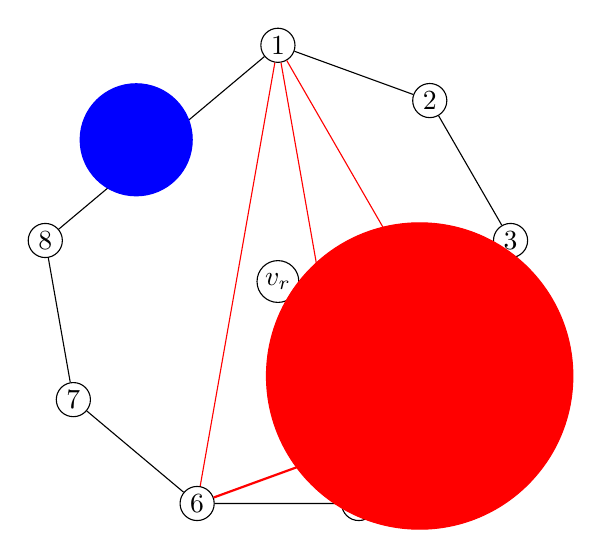
\begin{tikzpicture}[scale=1.2, every node/.style={circle, draw, fill=white, inner sep=1.5pt}]
        \foreach \i/\angle in {1/90,2/50,3/10,4/-30,5/-70,6/-110,7/-150,8/170} {
            \node (v\i) at (\angle:2.5) {\i};
        }
        \draw (v1)--(v2)--(v3)--(v4)--(v5)--(v6)--(v7)--(v8)--(v1);
        \draw[red] (v1)--(v4);
        \draw[red] (v1)--(v5);
        \draw[red] (v1)--(v6);
        \draw[red, thick] (v4)--(v6);
        \node at (0,0) {\(v_r\)};
        \node[red] at (1.5, -1) {generating chord \((v_r, v_5)\)};
        \node[blue] at (-1.5, 1.5) {conflict?};
    \end{tikzpicture}
    \caption{A generating chord \((v_r, v_j)\) might already exist in \(S\) from a previous face. 
    Unlike a non-root chord, it can be flipped away in a child, so the branch may still contain valid triangulations. 
    Thus we cannot prune based on a conflicting generating chord alone.}
    \label{fig:generating_chord_conflict}
\end{figure}

Consequently, to guarantee that every branch we explore can lead to valid triangulations, we must ensure that the \emph{root triangulation} of the face (the starting point of the local genealogical tree) does not contain any chord that conflicts with \(S\). 
In other words, we need a \textbf{safe root triangulation}.

\section{The Concept of a Safe Root Triangulation}
\label{sec:safe_root_concept}

\begin{definition}[Safe root vertex]
    \label{def:safe_root}
    Let \(F\) be a face (cycle) with vertices listed in counterclockwise order, and let \(S\) be the global chord set from previously processed faces. 
    A vertex \(r\) of \(F\) is called a \textbf{safe root vertex} if, when we construct the fan triangulation from \(r\) (i.e., add all chords \((r, v)\) for every vertex \(v\) of \(F\) that is not a neighbour of \(r\) on the cycle), none of these chords belongs to \(S\). 
    The corresponding fan triangulation is called a \textbf{safe root triangulation}.
\end{definition}

If we can find a safe root vertex for a face, then the root of its local genealogical tree is guaranteed to be compatible with all previously added chords. 
Moreover, because the root has the maximum number of generating chords, any conflict that appears later (in a non-root chord) can be safely pruned. 
Thus the existence of a safe root is essential for our algorithm.

\section{Two Fundamental Questions}
\label{sec:two_questions}

The above discussion raises two immediate questions:

\begin{enumerate}
    \item \textbf{Existence:} For any face in a biconnected plane graph, given an arbitrary set \(S\) of chords from previous faces (which are all inside the outer region of the face), does there always exist a safe root vertex? 
    If not, our algorithm would fail for some inputs.
    
    \item \textbf{Efficiency:} Assuming a safe root exists, can we find one in time \(O(n)\) (where \(n\) is the number of vertices of the face) without harming the overall \(O(1)\) amortised time per triangulation?
\end{enumerate}

The remainder of this chapter is devoted to answering the first question positively: we prove that every face in a biconnected plane graph contains at least two safe root vertices, regardless of the chords already present. 
The second question (efficiently finding a safe root) is addressed in Chapter~\ref{ch:safe_root_algorithm}.

\section{Existence of a Safe Root Vertex}
\label{sec:existence_proof}

We now prove that, under the planarity assumption, there is always at least one (in fact, at least two) vertex that can serve as a safe root.

\begin{theorem}[Existence of safe root vertices]
    \label{thm:safe_root_exists}
    Let \(F\) be a face (a simple cycle) of a biconnected plane graph \(G\), and let \(S\) be any set of chords that lie strictly outside \(F\) (i.e., in the region of the graph that has already been triangulated by previous faces). 
    Then there exist at least two vertices of \(F\) that are safe roots.
\end{theorem}

\begin{proof}
    We prove the theorem by induction on the number of vertices of \(F\) and on the structure of chords outside \(F\). 
    The key observation is that any chord in \(S\) that connects two vertices of \(F\) must lie entirely outside \(F\) (by planarity) and divides the cycle into two arcs. 
    Such a chord imposes constraints on which vertices can be safe roots.

    \begin{figure}[htbp]
        \centering
        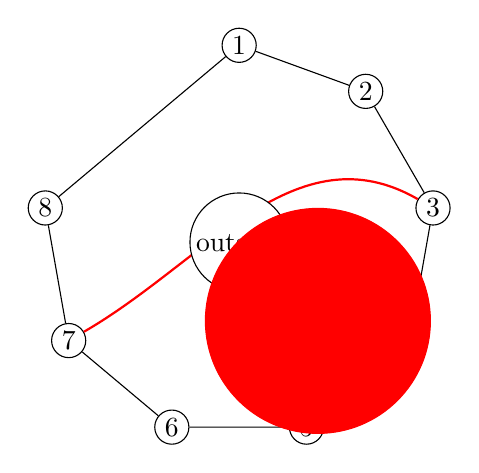
\begin{tikzpicture}[scale=1, every node/.style={circle, draw, fill=white, inner sep=1.5pt}]
            \foreach \i/\angle in {1/90,2/50,3/10,4/-30,5/-70,6/-110,7/-150,8/170} {
                \node (v\i) at (\angle:2.5) {\i};
            }
            \draw (v1)--(v2)--(v3)--(v4)--(v5)--(v6)--(v7)--(v8)--(v1);
            \draw[red, thick] (v3) to[out=150,in=30] (v7);
            \node at (0,0) {outside};
            \node[red] at (1, -1) {chord \((v_3, v_7) \in S\)};
        \end{tikzpicture}
        \caption{A chord \((v_i, v_j)\) outside the face divides the cycle into two arcs. No chord can cross this chord by planarity, so constraints are separated.}
        \label{fig:external_chord}
    \end{figure}

    Let the vertices of \(F\) be \(v_1, v_2, \dots, v_m\) in counterclockwise order. 
    If there is no chord in \(S\) connecting two vertices of \(F\), then every vertex is a safe root, and the theorem holds trivially.

    Otherwise, consider a chord \((v_i, v_j) \in S\) with \(i < j\). 
    This chord lies completely outside \(F\) (by definition of \(S\) as chords from previous faces, which are on the other side of \(F\)). 
    By planarity, any other chord in \(S\) that connects two vertices of \(F\) must lie entirely on one of the two arcs defined by \((v_i, v_j)\); it cannot cross \((v_i, v_j)\). 
    Thus \((v_i, v_j)\) separates the cycle into two independent subproblems.

    The two arcs are:
    \begin{itemize}
        \item The arc \(A_1 = v_i, v_{i+1}, \dots, v_j\) (including both endpoints)
        \item The arc \(A_2 = v_j, v_{j+1}, \dots, v_i\) (wrapping around)
    \end{itemize}
    Each arc, together with the chord \((v_i, v_j)\), forms a closed region (a smaller cycle) that is independent of the other. 
    Moreover, any chord in \(S\) that lies inside \(A_1\) (i.e., with both endpoints in \(A_1\)) can be considered as an external chord for the subface bounded by \(A_1\) and the chord \((v_i, v_j)\). 
    The same holds for \(A_2\).

    \begin{figure}[htbp]
        \centering
        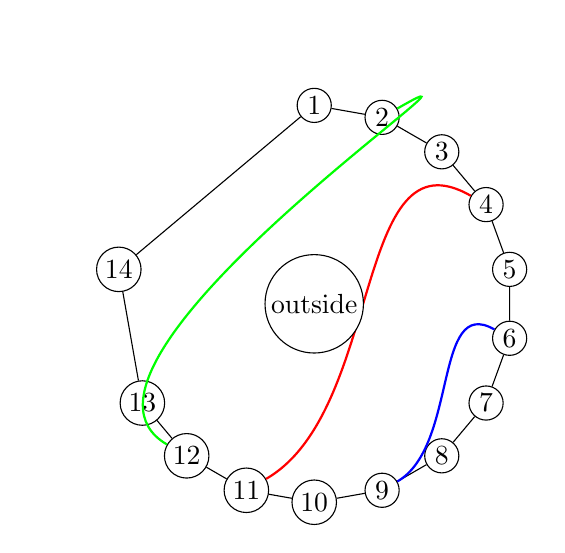
\begin{tikzpicture}[scale=0.9, every node/.style={circle, draw, fill=white, inner sep=1.5pt}]
            \foreach \i/\angle in {1/90,2/70,3/50,4/30,5/10,6/-10,7/-30,8/-50,9/-70,10/-90,11/-110,12/-130,13/-150,14/170} {
                \node (v\i) at (\angle:2.8) {\i};
            }
            \draw (v1)--(v2)--(v3)--(v4)--(v5)--(v6)--(v7)--(v8)--(v9)--(v10)--(v11)--(v12)--(v13)--(v14)--(v1);
            \draw[red, thick] (v4) to[out=150,in=30] (v11);
            \draw[blue, thick] (v6) to[out=150,in=30] (v9);
            \draw[green, thick] (v12) to[out=150,in=30] (v2);
            \node at (0,0) {outside};
        \end{tikzpicture}
        \caption{Multiple external chords partition the face into independent segments. 
        Each segment can be treated separately; a safe root can be found in each segment, and the endpoints of the segment are potential safe roots for the whole face.}
        \label{fig:partition}
    \end{figure}

    By recursively applying this decomposition, we reduce the problem to finding a safe root in a smaller face that has no external chords (a ``primitive'' segment). 
    Therefore it suffices to prove that every primitive segment (a cycle with no chords from \(S\) inside it) contains at least two safe roots.

    Consider a primitive segment consisting of \(t\) vertices \(u_1, u_2, \dots, u_t\) in cyclic order, with the additional chord \((u_1, u_t)\) being the boundary of the segment (this chord may be an original edge of \(G\) or a chord from \(S\)). 
    Inside this segment there are no chords from \(S\). 
    We claim that at least two vertices among \(\{u_2, \dots, u_{t-1}\}\) are safe roots.

    The proof proceeds by induction on \(t\).

    \noindent\textbf{Base case: \(t = 3\) (a triangle).} 
    The segment has only three vertices. 
    The chord \((u_1, u_t)\) is already present. 
    The interior vertex \(u_2\) has degree 2 within the segment (connected to \(u_1\) and \(u_3\)), so it cannot have any chord to a non-neighbour (there are none). 
    Thus \(u_2\) is a safe root. 
    Similarly, if the triangle is isosceles, both \(u_1\) and \(u_3\) are also safe? Actually \(u_1\) and \(u_3\) have the chord \((u_1, u_3)\) already present, so they are not safe because adding \((u_1, u_3)\) would create a multi-edge. 
    So only \(u_2\) is safe, but we need two? Wait, the theorem claims at least two safe roots for the whole face, not necessarily for a primitive segment. 
    For a primitive segment that is a triangle, there is exactly one vertex that is not an endpoint of the external chord. 
    That vertex is safe. 
    However, the whole face consists of many such segments concatenated; the endpoints of segments (which are vertices of the original face) may be safe when considering the whole face. 
    The induction will accumulate safe roots.

    Actually, the standard proof (as in the author’s original text) uses the notion of \(T_n\) structures. 
    Let us follow that argument directly.

    \begin{figure}[htbp]
        \centering
        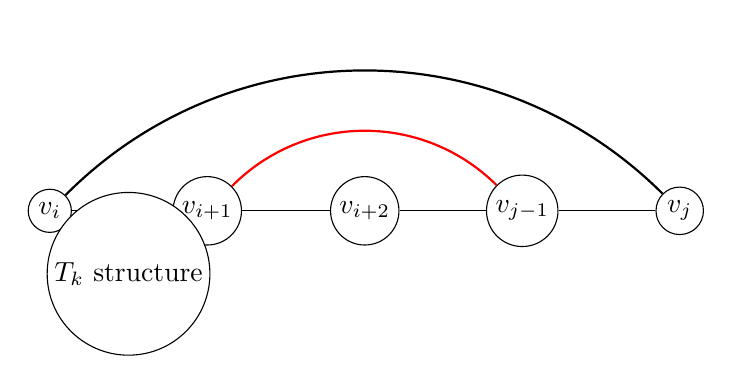
\begin{tikzpicture}[every node/.style={circle, draw, fill=white, inner sep=2pt}]
            \node (v1) at (0,0) {\(v_i\)};
            \node (v2) at (2,0) {\(v_{i+1}\)};
            \node (v3) at (4,0) {\(v_{i+2}\)};
            \node (v4) at (6,0) {\(v_{j-1}\)};
            \node (v5) at (8,0) {\(v_j\)};
            \draw (v1)--(v2)--(v3)--(v4)--(v5);
            \draw[thick, bend left=45] (v1) to (v5);
            \draw[red, thick, bend left=45] (v2) to (v4);
            \node at (1, -0.8) {\(T_k\) structure};
        \end{tikzpicture}
        \caption{A \(T_k\) structure: a path of vertices with a chord connecting the endpoints, and possibly additional chords inside. 
        The induction shows that at least one vertex among the interior ones is safe.}
        \label{fig:Tk_structure}
    \end{figure}

    Define a \(T_k\) structure as a set of vertices \(\{v_i, v_{i+1}, \dots, v_j\}\) such that:
    \begin{itemize}
        \item The boundary edges \((v_i, v_{i+1}), \dots, (v_{j-1}, v_j)\) are part of the cycle or already added chords.
        \item There is a chord \((v_i, v_j)\) in \(S\) (or a boundary edge of the segment) that lies outside the face.
        \item All chords from \(S\) with both endpoints in this set lie strictly inside the region bounded by the path and the chord \((v_i, v_j)\).
    \end{itemize}
    A \(T_k\) structure has \(k+1\) vertices? In the original text, \(T_n\) refers to a structure with \(n\) vertices along the path. 
    We prove by induction on the number of interior vertices that there is at least one safe root.

    \textbf{Base case: \(T_1\) structure.} 
    This consists of three vertices \(v_i, v_{i+1}, v_j\) with \(j = i+2\). 
    The vertex \(v_{i+1}\) has no chords to any non-neighbour (its only neighbours are \(v_i\) and \(v_j\)), so it is a safe root.

    \textbf{Inductive step: \(T_k\) structure with \(k \ge 2\).} 
    Consider the vertex \(v_{i+1}\). 
    Its neighbours on the path are \(v_i\) and \(v_{i+2}\). 
    It could have chords to vertices \(v_{i+3}, v_{i+4}, \dots, v_j\) (since these are non-neighbours). 
    There are two cases:
    \begin{enumerate}
        \item \textbf{\(v_{i+1}\) has no chord to any vertex beyond \(v_{i+2}\).} 
        Then \(v_{i+1}\) itself is a safe root, because none of the chords from \(v_{i+1}\) to non-neighbours are present in \(S\). 
        The chord \((v_i, v_j)\) does not involve \(v_{i+1}\), so no conflict arises.
        
        \item \textbf{\(v_{i+1}\) has a chord to some vertex \(v_p\) with \(p \ge i+3\).} 
        This chord, together with the existing chord \((v_i, v_j)\), creates a smaller \(T_{k'}\) structure with \(k' < k\) (for example, between \(v_{i+1}\) and \(v_p\) or between \(v_p\) and \(v_j\)). 
        By the induction hypothesis, this smaller structure contains a safe root. 
        Moreover, that safe root is also a safe root for the original \(T_k\) structure, because any chord from it to a non-neighbour would have to lie inside the smaller structure and thus is already accounted for.
    \end{enumerate}
    In both cases, a safe root exists within the \(T_k\) structure.

    Since the whole face can be partitioned by the chords in \(S\) into a sequence of \(T_{k_1}, T_{k_2}, \dots, T_{k_m}\) structures (each corresponding to a maximal interval of vertices between two consecutive external chords), and each \(T_{k_\ell}\) structure contains at least one safe root, the entire face contains at least \(m\) safe roots. 
    Because the face is a cycle, there are at least two such intervals (one on each side of any external chord), so \(m \ge 2\). 
    Hence there are at least two safe root vertices for the whole face.
\end{proof}

\begin{remark}
    The proof is constructive: it shows how to locate safe roots by examining the structure of external chords. 
    In Chapter~\ref{ch:safe_root_algorithm} we give an explicit \(O(n)\) algorithm to find one safe root without explicitly constructing the \(T_k\) decomposition.
\end{remark}

\section{Implications for the Algorithm}
\label{sec:existence_implications}

Theorem~\ref{thm:safe_root_exists} guarantees that we can always start the triangulation of a face with a safe root triangulation, provided we have correctly maintained the global chord set \(S\) of previously added chords. 
Thus the root of the local genealogical tree will be compatible with all earlier faces. 
Any conflict that later appears will involve a non-root chord (since generating chords are, by construction, all safe at the root), and such conflicts can be safely pruned as described in Chapter~\ref{ch:pruning_strategy}.

The remaining task is to find a safe root vertex efficiently (in \(O(n)\) time) so that the total building cost per face does not exceed the number of triangulations generated. 
This is the subject of Chapter~\ref{ch:safe_root_algorithm}.

\section{Summary}
\label{sec:chapter8_summary}

We have identified a critical issue: generating chords themselves can conflict with previously added chords, but we cannot prune branches based on such conflicts because generating chords can be flipped away. 
To overcome this, we introduced the concept of a \emph{safe root triangulation} — a root of the local genealogical tree whose generating chords are all conflict-free. 
We proved that every face in a biconnected plane graph contains at least two safe root vertices, regardless of the chords already present from previous faces. 
This existence result ensures that our algorithm can always initialise the local tree safely. 
The next chapter provides an efficient method to find a safe root in linear time.